\chapter{Background and Preliminaries\label{chap:background}}
\localtoc

% Content:
% - Introduction to ML for IDS
%   - Supervised learning
%   - Unsupervised learning
%   - Metrics
%   - Datasets
% - Collaboration in IDS
%   - Centralized IDS
%   - Distributed IDS
%   - Collaborative IDS

\section{Introduction\label{sec:bg.intro}}

This chapter provides the necessary background and preliminaries to understand the rest of the thesis. 
We start by laying out the basics of \gls{ml} for intrusion detection in \Cref{sec:bg.ids}, followed by the implications of scaling up to \glspl{cids} in \Cref{sec:bg.collab}, enumerating along the way the challenges that motivate the use of \gls{fl}.
We then introduce the fundamentals of \gls{fl} in \Cref{sec:bg.fl}, focusing on the FedAvg algorithm and the notations used throughout the thesis.
Finally, we discuss the threats against \gls{fl} in \Cref{sec:bg.threats}, with a particular focus on data poisoning attacks.



\section{Intrusion Detection\label{sec:bg.ids}}

Organizations long relied on signature-based \glspl{ids} to detect intrusions.
These systems leverage a database of known attack patterns (\ie, \emph{signatures}) to identify malicious activities.
\Cref{lst:suricata} displays an example of a signature for detecting the Heartbleed vulnerability using Suricata~\cite{suricata}, a popular open-source \gls{ids}.
This signature relies on dedicated code inside Suricata's engine that required extensive human intervention to develop.
It is consequently specific to Suricata and remains difficult to interpret and adapt.
Such limitations motivated the study of \gls{ml} for automatically extracting patterns from data, enabling the development of more flexible and adaptive \glspl{ids}.

\begin{listing}
  \begin{lstlisting}[gobble=4]
    alert tls any any -> any any (msg:"SURICATA TLS overflow heartbeat encountered, possible exploit attempt (heartbleed)"; flow:established; app-layer-event:tls.overflow_heartbeat_message; flowint:tls.anomaly.count,+,1; classtype:protocol-command-decode; reference:cve,2014-0160; sid:2230012; rev:1;)
  \end{lstlisting}
  \caption[
    Example of a Suricata signature for detecting the Heartbleed vulnerability.
  ]{
    Example of a Suricata signature for detecting the Heartbleed vulnerability\footnotemark{}.
    \label{lst:suricata} 
  }
\end{listing}

\footnotetext{\url{https://github.com/OISF/suricata/blob/master/rules/tls-events.rules}}

\Glspl{ids} can be broadly classified into two categories: \emph{misuse detection} and \emph{anomaly detection}.
Misuse detection refers to the identification of known attack patterns.
Signature-based \glspl{ids} fall into this category.
On the other hand, anomaly detection compares a normal profile (trained on nominal traffic) with observed events to determine if they are malicious~\cite{garcia-teodoro_Anomalybasednetworkintrusion_2009}.
This approach is \emph{de facto} more efficient for detecting novel attacks, but it is also more prone to false positives.

An analogy can be drawn between this classification and the two main paradigms of \gls{ml}: supervised and unsupervised learning.
In supervised learning, the model is trained on labeled data, where each sample is associated with a label.
Labels can be classes (binary or multi-class classification) or continuous values (regression).
Either way, the model's objective is to predict the label of unseen samples.
In unsupervised learning, no labels are provided.
The model's goal is to find patterns in the data, such as clusters or outliers.
In anomaly detection, the model is trained on normal data only, and its objective is to detect deviations from this normal profile.

Multiple \gls{ml} algorithms have been applied to intrusion detection, including \glspl{svm}, \glspl{rf}, and \glspl{ann}.
However, the rise of \gls{dl} has led to a significant improvement in the performance of \glspl{ids}.
\Gls{dl} is a subfield of \gls{ml} that focuses on learning representations of data through the use of neural networks.
In the following sections, we introduce the basics of \gls{dl} for intrusion detection, review the existing paradigms, and discuss the metrics and datasets used to evaluate these systems.


\subsection{Deep Learning for Intrusion Detection\label{sec:bg.ids.dl}}

\Gls{dl} present several advantages over traditional \gls{ml} algorithms.
Most notably, they automatically learn features from the data, reducing the need for manual feature engineering.
This is particularly useful in the context of intrusion detection, where the features are often complex, interdependent, and of unequal relevance.
The training data can range from network traffic to system logs depending on the type of mechanism used: network-based, host-based, or hybrid.
Yet, \glspl{nids} greatly outnumber other approaches in the literature, due the availability of network traffic datasets and the ease of deployment.

Most of the research on \gls{nids} use a representation known as \emph{unidirectional network flows} or \emph{netflows}, where a flow is defined as a sequence of packets sharing the same source and destination addresses, ports, and protocol.
Various features can be extracted from these flows, such as the number of packets, bytes, and the duration of the flow.
More details on the features used in \gls{nids} can be found in \Cref{sec:bg.ids.datasets}.
More generally, the dataset $D$ of size $n$ is represented as a set of variables $X_i = \langle x_1, x_2, \ldots, x_m \rangle, i \in \llbracket 1, n \rrbracket $, where $x_j$ corresponds to the $j$-th feature, and $m$ to the number of features.

\begin{figure}
  \centering
  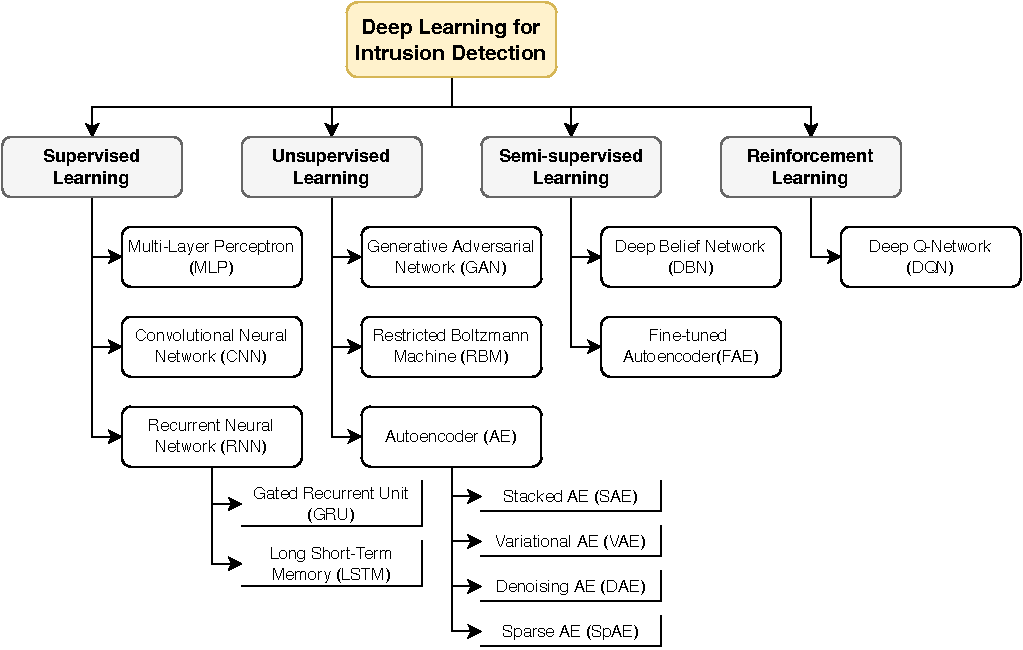
\includegraphics[width=0.8\textwidth]{figures/ml-taxonomy.pdf}
  \caption{
    Taxonomy of the main \gls{dl} paradigms.
    \label{fig:bg.taxonomy}
  }
\end{figure}

\subsubsection{Main \Gls{dl} Paradigms}

Because of their layered architecture, \glspl{dnn} can adopt different forms depending on the type of input data and the task at hand.
\Cref{fig:bg.taxonomy} presents the major families of \gls{dl} algorithms: supervised, unsupervised, and semi-supervised learning, and finally reinforcement learning.
While works exist on the application of reinforcement learning to intrusion detection~\cite{he_ReinforcementLearningMeets_2024}, they remain rare in the literature.
Consequently, we focus on supervised and unsupervised learning in this thesis.
This section provides an overview of these paradigms, and define for each the learning problem in the context of intrusion detection.

\paragraph{Supervised Learning}

\begin{figure}
  \captionsetup{justification=justified,singlelinecheck=false}
  \centering
  \begin{subfigure}{\textwidth}
    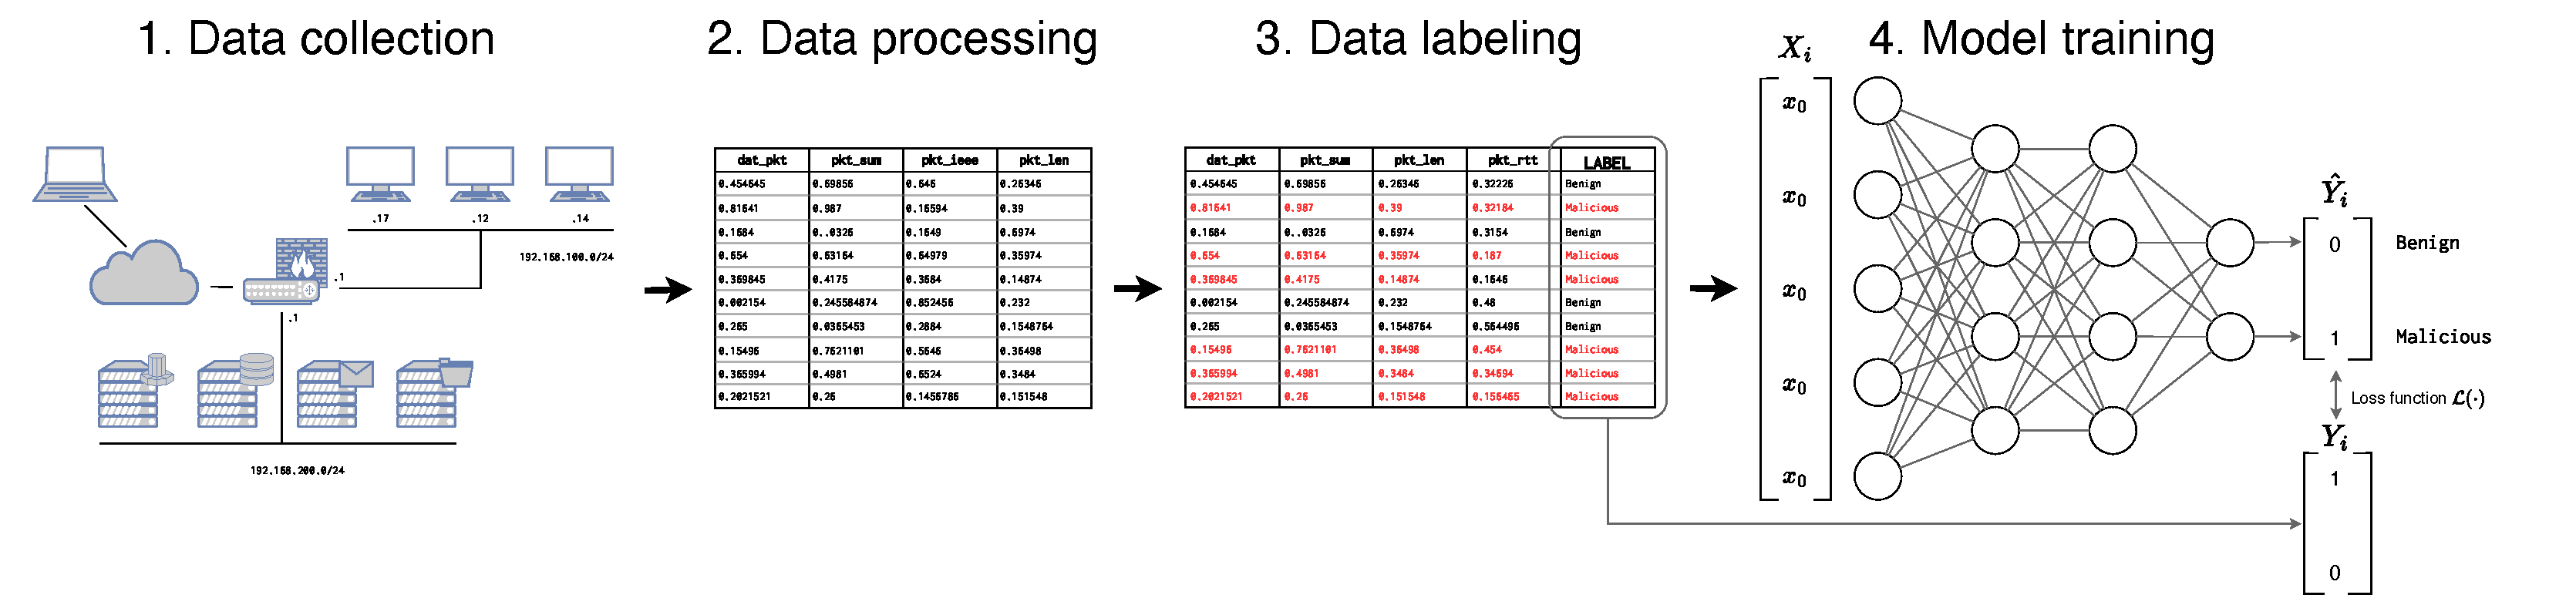
\includegraphics[width=\textwidth]{figures/mlp-train.drawio.pdf}
    \caption{
      Training phase.
      \label{fig:bg.mlp.train}
    }
  \end{subfigure}
  \begin{subfigure}{\textwidth}
    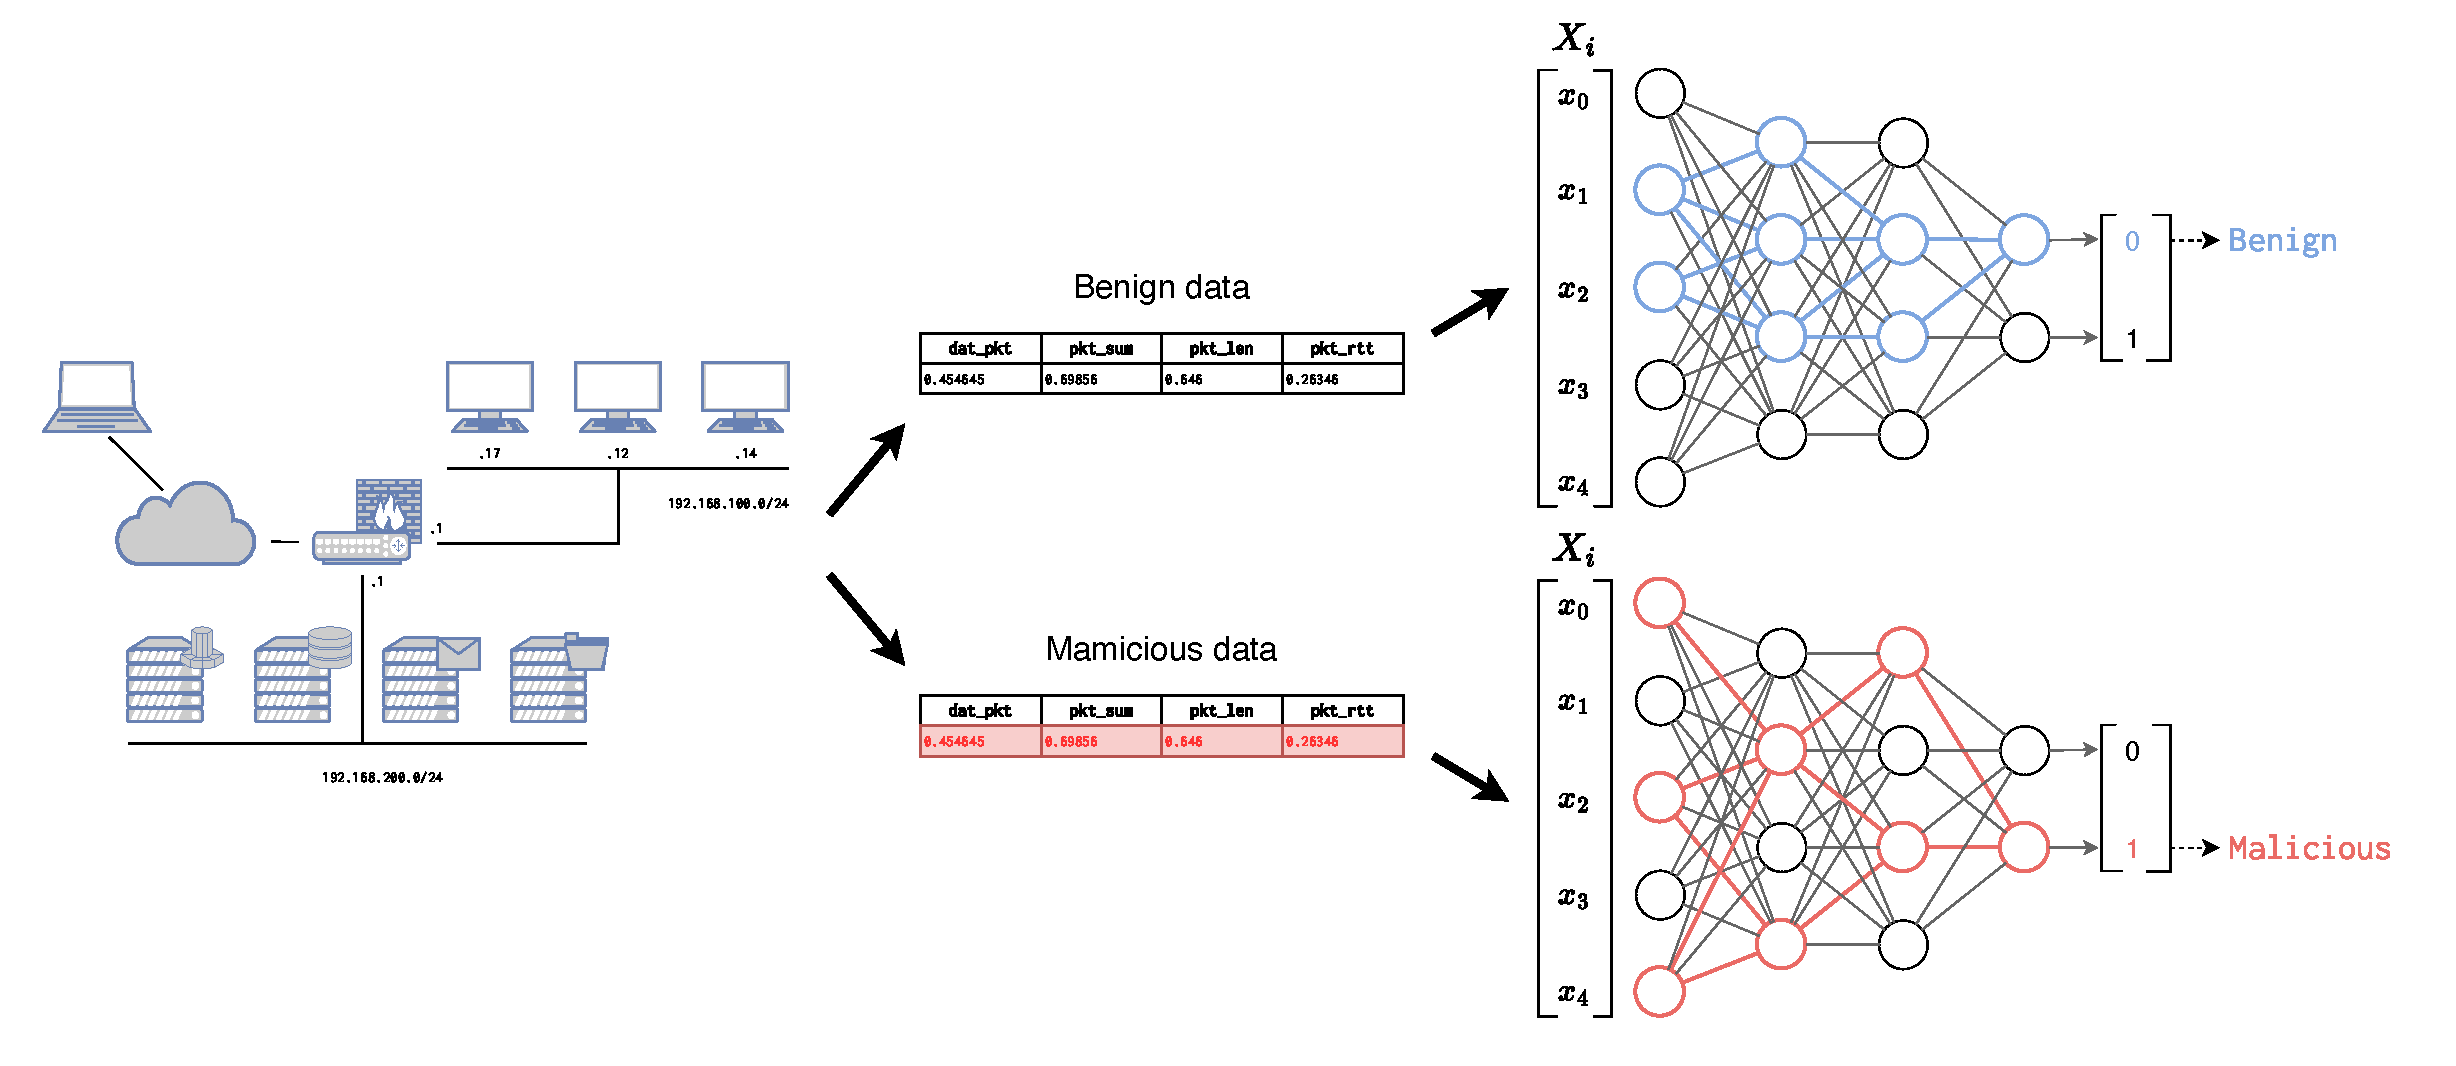
\includegraphics[width=.75\textwidth,left]{figures/mlp-predict.drawio.pdf}
    \caption{
      Prediction phase.
      \label{fig:bg.mlp.predict}
    }
  \end{subfigure}
  \caption{
    Workflow of a \acrfull{mlp} for intrusion detection.
    \label{fig:bg.mlp}
  }
\end{figure}

Supervised learning is the most common approach in \gls{ml}, and refers to the training of a model on labeled data.
In the context of \glspl{ids}, practitioners usually seek to classify network flows into two classes (\emph{benign} and \emph{malicious}), which is a binary classification task.
Consequently, the dataset $D$ of size $n$ associates each sample $X_i$ with a label $y_i \in \lbrace 0,1 \rbrace $.
The model is trained to predict the label $\hat{y}$ of unseen samples.
To do so, we generally use a \gls{sgd}-based optimizer to minimize a loss function
\begin{equation} \label{eq:bg.loss}
  \mathcal{L}(w, X_i, y_i), i \in \llbracket 1, n \rrbracket,
\end{equation}
where $w$ represent the model's parameters.
After computing the gradients $\nabla \mathcal{L}(w, X_i, y_i)$, they can update their model as
\begin{equation} \label{eq:bg.update}
  w^{t+1} \gets w^t - \eta \nabla \mathcal{L}(w, X_i, y_i),
\end{equation}
where $\eta$ is the learning rate, $w^t$ the model's parameters at iteration $t$, and $w^{t+1}$ the new parameters resulting from the update.
The last layer usually uses \texttt{softmax} or \texttt{sigmoid} activation functions to output a probability of being in a class (normal or abnormal).
In the case of multi-class classification, the label is one-hot encoded\footnotemark{} into a vector $Y$ of size $c$ (the number of classes), and the \texttt{softmax} function is used.
Depending on the available features and the learning objective, various architectures can be used, such as \glspl{cnn} for high-dimensional data, or \glspl{rnn} for sequential data.
\Glspl{mlp} are the simplest and most common architecture used in \gls{ids}, and the one that we focus on in this thesis, although most concepts can be extended to other architectures.

\footnotetext{
  One-hot encoding is a binary representation of categorical variables, where each category is mapped to a binary vector.
  It is typically used in \gls{ml} to represent categorical data, such as the protocol type in netflows.
}

One of the main challenges in supervised learning is the availability of labeled data and its quality.
In the context of \gls{ids}, obtaining enough labeled data is particularly challenging, as labeling requires expert knowledge and is time-consuming.
Moreover, the class distribution is often unbalanced, with benign traffic being much more frequent than anomalies in the testing set~\cite{chandola_Anomalydetectionsurvey_2009}.
This issue is aggravated in siloed configurations, \ie, in which models can only be trained on locally-collected data.
This can lead to models that are skewed by the unbalanced class distribution~\cite{campos_EvaluatingFederatedLearning_2022}.

\begin{challenge}
  Locally collected data is often unbalanced, leading to representation biases and overall lower performance.
  \label{chall:bias}
\end{challenge}


\paragraph{Unsupervised Learning}

\begin{figure}
  \captionsetup{justification=justified,singlelinecheck=false}
  \centering
  \begin{subfigure}{\textwidth}
    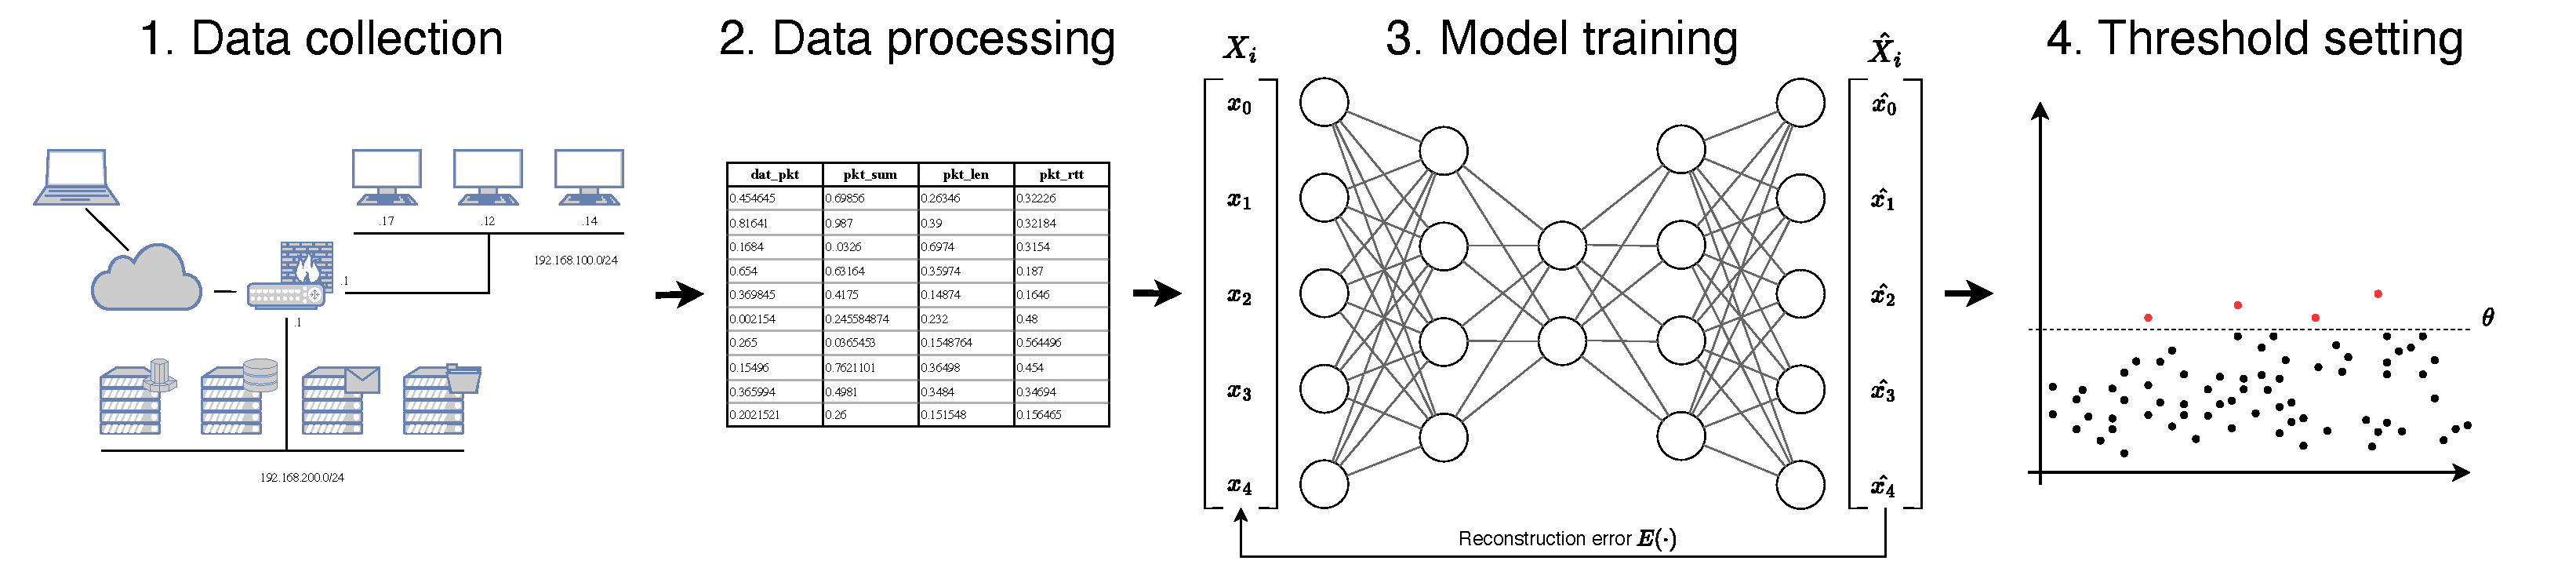
\includegraphics[width=\textwidth]{figures/ae-train.drawio.pdf}
    \caption{
      Training phase.
      \label{fig:bg.ae.train}
    }
  \end{subfigure}
  \begin{subfigure}{\textwidth}
    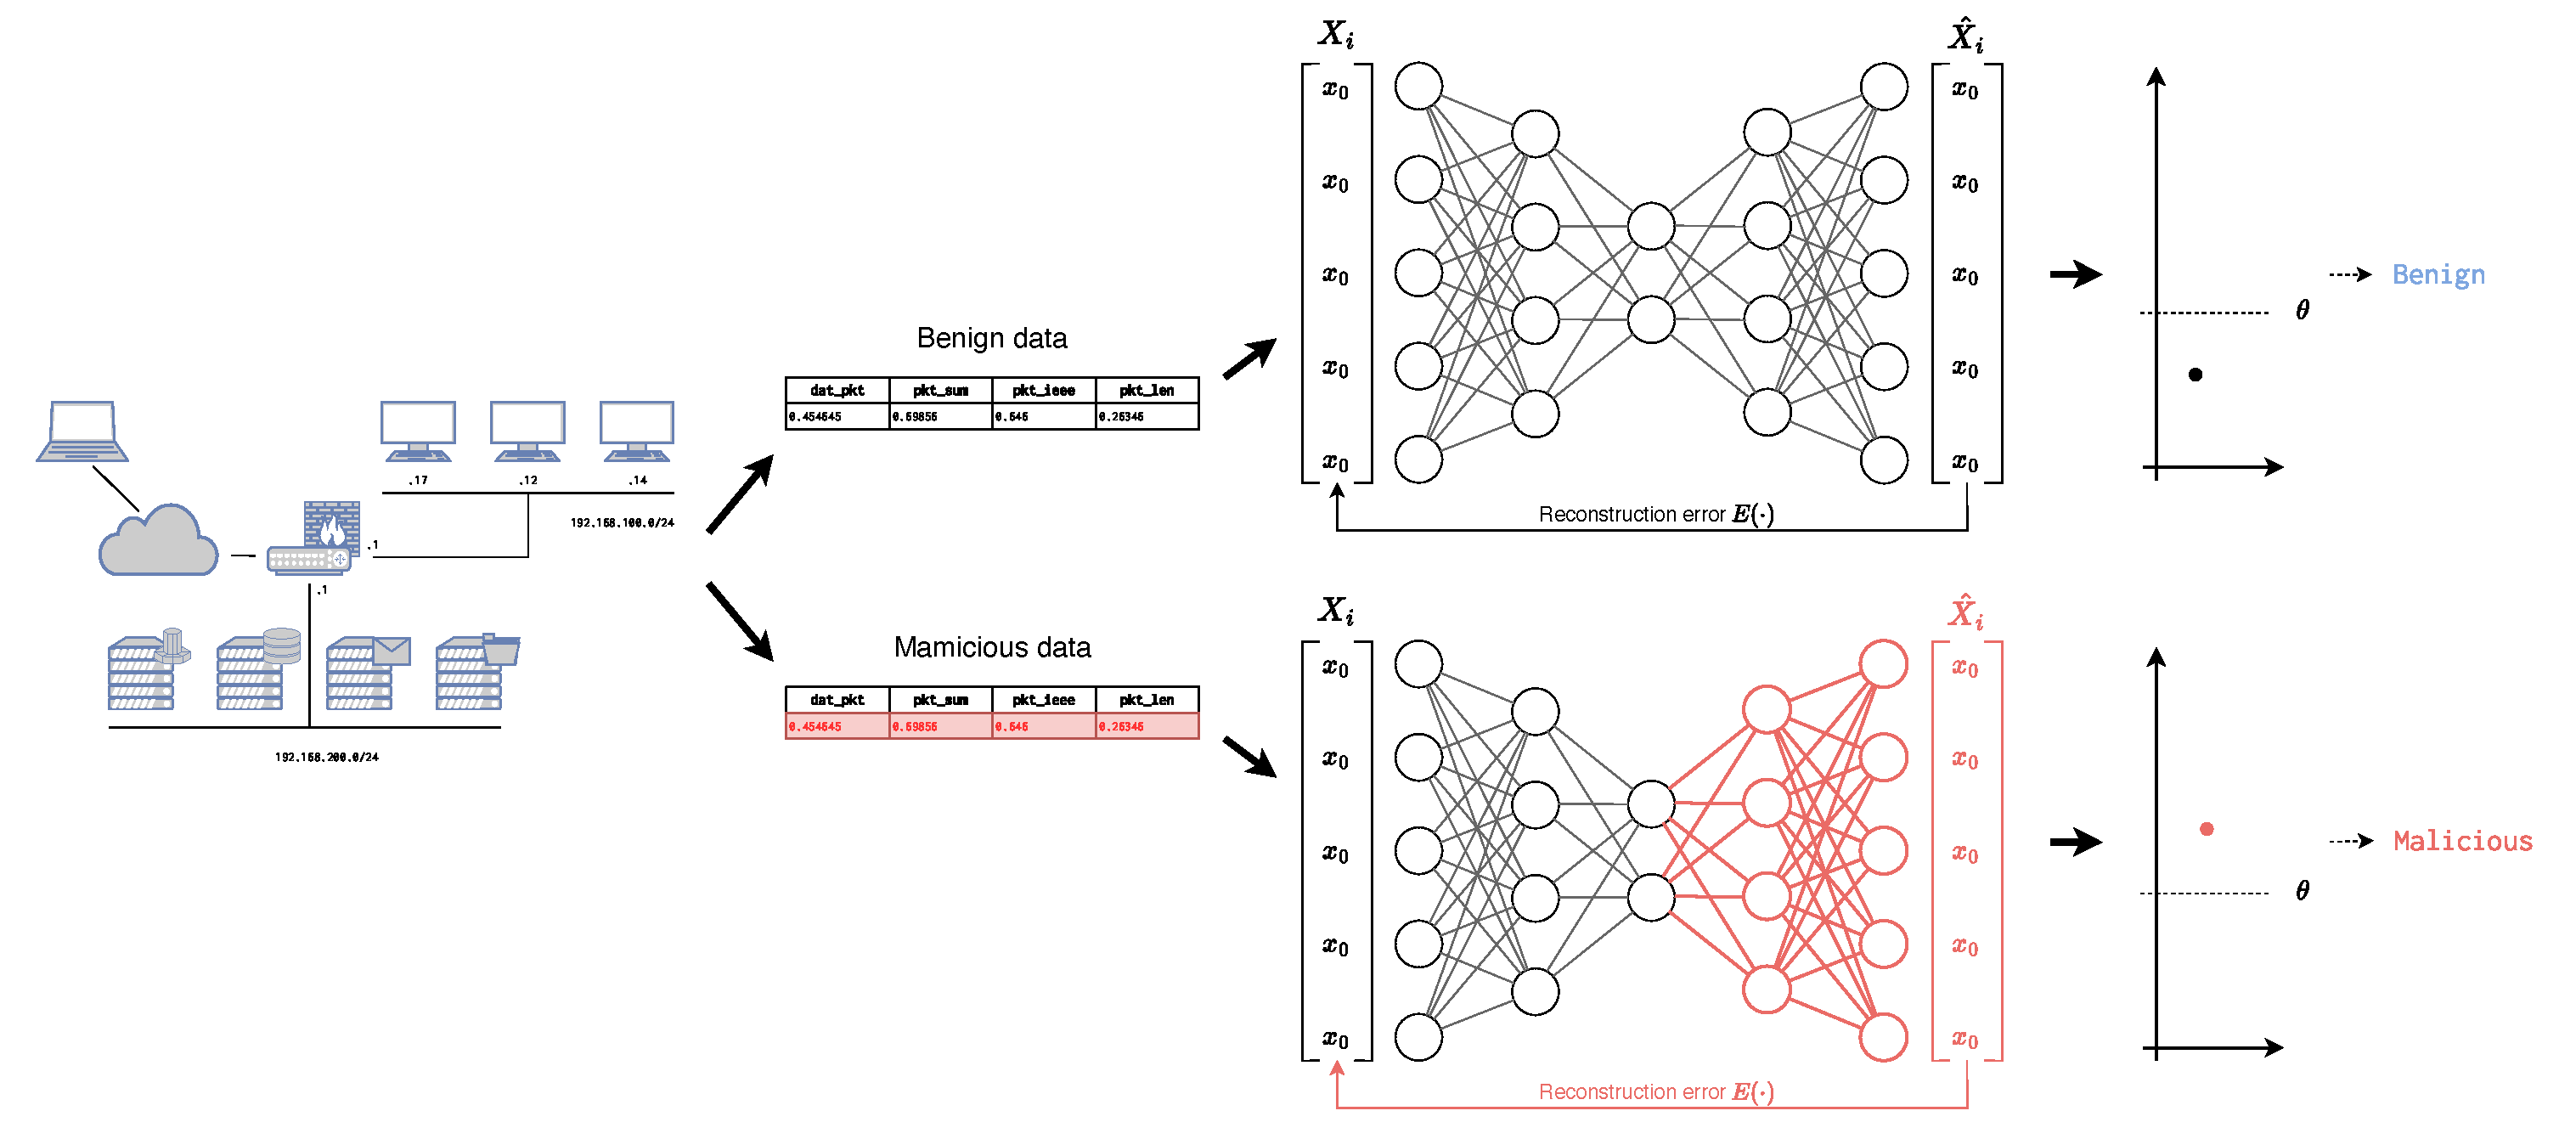
\includegraphics[width=.75\textwidth,left]{figures/ae-predict.drawio.pdf}
    \caption{
      Prediction phase.
      \label{fig:bg.ae.predict}
    }
  \end{subfigure}
  \caption{
    Workflow of a \acrfull{sae} for intrusion detection.
    \label{fig:bg.ae}
  }
\end{figure}

To circumvent the need for labeled data, unsupervised learning can be used.
Unsupervised \gls{ml} algorithms are typically used for clustering or outlier detection.
The \gls{dl} variants are rather used for feature extraction and dimensionality reduction, or anomaly detection.
To detect anomalies, \glspl{ae} can be trained on normal data only, and then used to see whether the reconstruction error of a new sample is above a certain threshold.
This builds on the assumption that
\begin{enumerate*}[(i)]
  \item benign traffic is much more frequent that anomalies in the testing set~\cite{chandola_Anomalydetectionsurvey_2009}; and
  \item abnormal packets are statistically different from normal ones.
\end{enumerate*}
In this scenario, the training dataset $D$ is composed of benign (\ie, normal) samples only and no associated label.
Given $\mathcal{X} = \langle X_i | i \in \llbracket 1, n \rrbracket \rangle $, the model is trained to minimize the reconstruction error $\mathcal{L}(\mathcal{X}, \hat{\mathcal{X}})$, where $\hat{\mathcal{X}}$ is the output of the \gls{ae}.
A typical error function for this task is the \gls{mse}, expressed as:
\begin{equation}
  \text{MSE} = \frac{1}{n} \sum_{i=1}^{n} \left( X_i - \hat{X}_i \right)^2.
\end{equation}
Then the model can be updated using the same process described in \Cref{eq:bg.update}.
Different architectures of \glspl{ae} can be used, such as \glspl{sae} to improve the quality of the extracted features, or \glspl{dae} to improve the robustness of the model~\cite{gjorgiev_TimeSeriesAnomaly_2020}. 
To detect anomalies, the reconstruction error of a new sample is compared to a threshold $\theta$ defined during the training phase on validation data.
A high reconstruction error indicates that the considered samples is too \emph{far} from the training data, and can indicate an anomaly.
The performance of the combination of the \gls{ae} and the threshold can then be evaluated using a labelled test set.

While unsupervised learning is particularly useful for detecting novel attacks, it is also more prone to misclassification.
Local data in the real-world is likely to be collected on devices with little variance, \eg same brand, same protocols, or use cases.
This can lead to a normal profile that is too specific to the local environment, and thus would raise alerts as soon as a change occurs~\cite{liu_MachineLearningDeep_2019}.

\begin{challenge}
  Local data is specific to the environment, increasing the risk of false positives when changes occur.
  \label{chall:specificity}
\end{challenge}


\paragraph{Semi-supervised Learning}

Semi-supervised learning is a hybrid approach where only a small part of the training data is labeled.
This approach is particularly useful in the context of \gls{ids}, where labeled data is scarce.
A common strategy is to train an \gls{ae} on the full dataset to learn the optimal representation of the data, and use the encoder (see \Cref{fig:bg.ae}) part with a classifier to predict the label of the samples~\cite{aouedi_SemisupervisedStackedAutoencoder_2020}.
Other known model architectures for semi-supervised learning include \glspl{dbn}, where multiple layers of \glspl{rbm} are stacked to form a deep network that extracts features from the data.
The model is then fine-tuned using the labeled data for classification purposes.


\subsection{Datasets\label{sec:bg.ids.datasets}}

Datasets are essential in intrusion detection, as they allow researchers to evaluate and compare their solutions.
This is even more critical when leveraging \gls{ml} and \gls{dl} techniques, as the performance of these models is highly dependent on the quality and quantity of the training data.
Until the mid-2010s, the most common dataset used for intrusion detection was the {KDD'99} dataset~\cite{kddcup99}, built for the KDD Cup 1999 competition using the DARPA 1998 dataset.
\Textcite{tavallaee_detailedanalysisKDD_2009} published an updated version of the dataset, called NSL-KDD, which removes duplicates and corrects some errors in the original dataset.
However, NSL-KDD is still based on the original DARPA 1998 dataset, and is considered outdated by today's standards.

Since 2015 with the publication of the UNSW-NB15 dataset~\cite{moustafa_UNSWNB15comprehensivedata_2015}, new datasets have been developed to address the limitations of the KDD'99 and NSL-KDD datasets, such as the lack of realism\footnotemark{} of the generated traffic, the lack of attack diversity, and the scale of the experiments.
\Cref{tbl:datasets} presents the most common feature-based datasets for \glspl{nids}, along with their characteristics.
Two teams have been particularly active in this area: the Intelligent Security Group (ISG)~\cite{moustafa_UNSWNB15comprehensivedata_2015,koroniotis_developmentrealisticbotnet_2019,moustafa_newdistributedarchitecture_2021} at the University of New South Wales, Australia, and the Canadian Institute for Cybersecurity (CIC)~\cite{sharafaldin_GeneratingNewIntrusion_2018} at the University of New Brunswick, Canada.
They brought the most used datasets in the field in recent years, UNWS-NB15 and CICIDS2017, respectively.

\footnotetext{
  Only in regard to modern networks.
  Indeed, the DARPA 1998 dataset simulates multiple workstations in a military environment, using the US Air Force Research Laboratory's testbed.
  The technologies deployed where representative of the state of the art at the time.
}

\begin{table}
  \centering
  \caption{
    Most common feature-based datasets for \glspl{nids}.
    \label{tbl:datasets}  
  }
  \hfill
\begin{minipage}{.48\textwidth}
  \small
  \begin{tabularx}{\linewidth}{lXrr}
    \toprule % ------------------------------------
    \multicolumn{1}{c}{\textbf{Class}} & & \multicolumn{1}{c}{\textbf{Sampled}} & \multicolumn{1}{c}{\textbf{Full}} \\
    \midrule % ---------------------------------
    Benign         & & 880,623   & 16,635,567 \\
    DDoS           & & 73,558    & 1,390,270  \\
    DoS            & & 25,574    & 483,999    \\
    Bot            & & 7,595     & 143,097    \\
    Brute Force    & & 6,525     & 123,982    \\
    Infiltration   & & 6,108     & 116,361    \\
    Injection      & & 17        & 432        \\
    & & & \\
    & & & \\
    & & & \\
    \midrule % ---------------------------------
    \textbf{Total} & & 1,000,000 & 18,893,708 \\
    \bottomrule % ---------------------------------
  \end{tabularx}
\end{minipage}
\hfill
\begin{minipage}{.48\textwidth}
  \small
  \begin{tabularx}{\linewidth}{lXrr}
    \toprule % ---------------------------------
    \multicolumn{1}{c}{\textbf{Class}} & & \multicolumn{1}{c}{\textbf{Sampled}} & \multicolumn{1}{c}{\textbf{Full}} \\
    \midrule % ---------------------------------
    Benign           & & 960,078  & 2,295,222   \\
    Exploits         & & 13,187   & 31,551      \\
    Fuzzers          & & 9,377    & 22,310      \\
    Generic          & & 6,976    & 16,560      \\
    Reconnaissance   & & 5,352    & 12,779      \\
    DoS              & & 2,455    & 5,794       \\
    Analysis         & & 969      & 2,299       \\
    Backdoor         & & 925      & 2,169       \\
    Shellcode        & & 617      & 1,427       \\
    Worms            & & 64       & 164         \\
    \midrule % ---------------------------------
    \textbf{Total}   & & 1,000,000 & 2,390,275  \\
    \bottomrule % ------------------------------
  \end{tabularx}
\end{minipage}
\hfill
  \end{table}

\paragraph{Provided features}

Because most of the datasets presented in \Cref{tbl:datasets} are made to train and evaluate \glspl{ml} models, they rely on a set of features extracted from the network traffic.
Some also include the original network captures (PCAPs) for further analysis, or complementary system logs for correlation purposes.
Two non-exclusive approaches can be used to produce these features: feature extraction and feature selection.

\begin{description}[labelindent=1em]
  \item[Feature extraction:] It refers to the computation of numerical characteristics after the data collection; \eg, \gls{iat} or number of packets per device in the context of traffic monitoring.
  Most modern dataset use existing \glspl{ids} to extract these features, such as Zeek\footnote{Formerly known as Bro, available at: \url{https://www.zeek.org/}} or Argus\footnote{Available at: \url{https://openargus.org/argus-ids}}.
  The resulting data are network flows, aggregating the information of multiple packets into a single record.

  \item[Feature selection:] It relates to the selection of the relevant features for a given task.
  This is particularly useful in the context of \gls{ml}, where irrelevant or redundant features can degrade the performance of the model.
  For instance, Edge-IIoTset~\cite{ferrag_EdgeIIoTsetNewComprehensive_2022} contains 61 features, selected from a pool of 1176 using feature correlation.
\end{description}

The choice of features is critical for the performance of the model, although \gls{dl} models make this process less relevant due to their ability to filter out irrelevant features.
Yet, because each dataset comes with its own set of features, it is difficult to compare the performance of models across datasets.
Recently, \textcite{sarhan_StandardFeatureSet_2022} proposed a standardized feature set for intrusion detection based on NetFlow V9~\cite{rfc3954} format.
They used nProbe\footnote{Available at: \url{https://www.ntop.org/products/traffic-analysis/nprobe/}} to convert four known \gls{ids} datasets to this format: \ie, UNSW-NB15~\cite{moustafa_UNSWNB15comprehensivedata_2015}, Bot-IoT~\cite{koroniotis_developmentrealisticbotnet_2019}, ToN\_IoT~\cite{moustafa_newdistributedarchitecture_2021}, and CSE-CIC-IDS2018~\cite{sharafaldin_GeneratingNewIntrusion_2018}.
The converted datasets (that the author call NF-V2) contain 43 features extracted from flow characteristics, such as duration or packet length, and some others that are protocols-specific.
The uniform feature set across datasets allows the evaluation of \gls{ml} models across independently generated datasets.

\paragraph{Use cases}

Until 2017 included, most datasets aim at simulating a \emph{typical} network environment, such as deployed in an organization.
This is the case for KDD'99, NSL-KDD, UNSW-NB15, and CIDDS 1 and 2, and CICIDS2017.
Since, the focus progressively shifts towards more specific use cases, notably with the generalization of \gls{iot} devices.
These datasets include protocols that are not present in traditional IT-oriented networks, such as MQTT or CoAP.
This is the case for Bot-IoT~\cite{koroniotis_developmentrealisticbotnet_2019}, ToN\_IoT~\cite{moustafa_newdistributedarchitecture_2021}, and Edge-IIoTset~\cite{ferrag_EdgeIIoTsetNewComprehensive_2022}.



% \footnote{\url{https://www.rfc-editor.org/rfc/rfc3954}} Netflow V9

\subsection{Metrics\label{sec:bg.ids.metrics}}

Most research on \gls{ml} for intrusion detection relies on the same set of metrics to assess, validate, and compare their solutions~\cite{chaabouni_NetworkIntrusionDetection_2019,faraj_Taxonomychallengesmachine_2020,buczak_SurveyDataMining_2016}.
Most of these metrics are derived from the confusion matrix (see \Cref{tbl:bg.conf}), which is a table that summarizes the performance of a classification model along the different classes.
To compute the confusion matrix, the model's predictions ($\hat{y}$) are compared to the true labels ($y$, the ground truth) of the samples.
All the metrics presented in this section are defined for binary classification, but can be extended to multi-class classification~\cite{buczak_SurveyDataMining_2016}.

\begin{table}
  \centering
  \newcommand{\mkblue}{\cellcolor{cyan!20}}
\newcommand{\mkgreen}{\cellcolor{green!20}}
\newcommand{\mkred}{\cellcolor{red!20}}
\newcommand{\mkyellow}{\cellcolor{yellow!20}}
\newcommand{\mkgray}{\cellcolor{gray!20}}
\newcommand{\lborder}[1]{\multicolumn{1}{|c}{#1}}
\newcommand{\borders}[1]{\multicolumn{1}{|c|}{#1}}
\newcommand{\mkcell}[2][c]{\renewcommand{\arraystretch}{1}\begin{tabular}{@{}#1@{}}#2\end{tabular}}

\renewcommand{\arraystretch}{3.3}
{\sffamily\selectfont\small%
\begin{tabular}{cccc}
  \cline{3-4}
  & & \multicolumn{2}{|c|}{\mkblue \textbf{Predicted condition}} \\
  \cline{2-4}
    & \lborder{\mkgray \mkcell{Total population \\ $= P + N$}} & \lborder{\mkblue Positive (PP)} & \borders{\mkblue Negative (PN)} \\
  \hline
  \lborder{\mkyellow} & \lborder{\mkyellow Positive (P)} & \lborder{\mkgreen \gls{tp}} & \borders{\mkred \gls{fn}} \\
  \cline{2-4}
  \lborder{\mkyellow \multirow{-2}{*}{\rotatebox{90}{\textbf{Actual condition}}}}%
    & \lborder{\mkyellow Negative (N)} & \lborder{\mkred \gls{fp}} & \borders{\mkgreen \gls{tn}} \\
  \hline
\end{tabular}
}
  \caption{
    Confusion matrix for binary classification.
    \label{tbl:bg.conf}
  }
\end{table}

\begin{enumerate}[(1)]
  \item \emph{Accuracy} represents the proportion of correctly classified items.
  It is the ability for the system to correctly distinguish abnormal traffic from legitimate one.
  \begin{equation*}
    \text{Accuracy} = \frac{\text{TP}+\text{TN}}{\text{P}+\text{N}}
  \end{equation*}

  \item \emph{Precision}, or \gls{ppv}, is the proportion of correct positive cases among all the cases that have been categorized as positive.
  \begin{equation*}
    \text{Precision} = \frac{\text{TP}}{\text{TP}+\text{FP}}
  \end{equation*}

  \item \emph{Recall}, or \gls{tpr} represents the proportion of true positive cases that have been correctly categorized.
  \begin{equation*}
    \text{Recall} = \frac{\text{TP}}{\text{P}} = \frac{\text{TP}}{\text{TP}+\text{FN}}
  \end{equation*}

  \item \emph{Specificity}, or \gls{tnr}, is the proportion of negative cases that has been correctly categorized.
  \begin{equation*}
    \text{Specificity} = \frac{\text{TN}}{\text{N}} = \frac{\text{TN}}{\text{TN}+\text{FP}}
  \end{equation*}

  \item \emph{Fallout}, or \gls{fpr}, represents the proportion of the positive cases that should have been categorized as negative.
  A high \gls{fpr} often requires human intervention after the classification task to filter out the false positive.

  \begin{equation*}
    \text{Fallout} = \frac{\text{FP}}{\text{N}} = \frac{\text{FP}}{\text{TN}+\text{FP}}
  \end{equation*}

  \item \emph{Missrate}, or \gls{fnr}, relates to the proportion of positive cases that have not been categorized as such.
  In the context of \glspl{ids}, it represents an attack that has been missed by the system.
  Thus, it is a critical metric for this use case.
  \begin{equation*}
    \text{Missrate} = \frac{\text{FN}}{\text{P}} = \frac{\text{FN}}{\text{TP}+\text{FN}}
  \end{equation*}

  \item \emph{F1-Score} is the harmonic mean of precision and recall.
  It is often used to measure ML algorithm, but is also criticized because of the equal importance it gives to both precision and recall~\cite{hand_noteusingFmeasure_2018}.
  \begin{equation*}
    F_1 = 2 \times \frac{\text{Precision} \times \text{Recall}}{\text{Precision}+\text{Recall}}
  \end{equation*}

  \item \emph{\gls{mcc}} is an adaptation of the \emph{Phi} (\(\phi\)) coefficient to confusion matrices.
  While being mathematically identical, the term is often preferred by the \gls{ml} community.
  The \gls{mcc} has significant advantages over the other metrics, as it covers all four categories of the confusion matrix~\cite{chicco_advantagesMatthewscorrelation_2020}.
  Thus, a high score can only be obtained with high \(\text{TP}\) and \(\text{TN}\), and low \(\text{FP}\) and \(\text{FN}\).

  \begin{equation*}
      MCC = \dfrac{
        \text{TP} \times \text{TN} - \text{FP} \times \text{FN}
      }{
        \sqrt{(\text{TP} + \text{FP})(\text{TN} + \text{FN})\cdot P \cdot N}
      }
  \end{equation*}%

\end{enumerate}
\section{Collaboration in Intrusion Detection\label{sec:bg.collab}}

The topic of collaboration in intrusion detection is rather old, with several surveys and reviews available in the literature~\cite{zhou_surveycoordinatedattacks_2010,elshoush_Alertcorrelationcollaborative_2011,vasilomanolakis_TaxonomySurveyCollaborative_2015,meng_CollaborativeSecuritySurvey_2015,folino_Ensemblebasedcollaborative_2016,li_SurveyingTrustBasedCollaborative_2022}, and the oldest references dating back to the early 1990s~\cite{snapp_DIDSdistributedintrusion_1992}.
In this section, we present the different types of collaboration in intrusion detection, and discuss some of the challenges that they face.
A first distinction can be made between their objectives, also they are not mutually exclusive:
\begin{enumerate*}[(i)]
  \item \emph{share results} to correlate alerts and detect attacks at a global scale, or
  \item \emph{share knowledge} to improve the detection capabilities of local systems.
\end{enumerate*}

This distinction also transpires from the scale of the collaboration.
The first case mostly refers to different probes, or sensors, that monitor the same infrastructure, and share their results to correlate alerts and detect attacks at the infrastructure level.
In the second case, which is sometimes referred to as a \gls{cidn}~\cite{li_SurveyingTrustBasedCollaborative_2022}, collaboration usually happens among different organizations or entities that monitor infrastructures.
In this thesis, we will focus on the latter, as it is more relevant to the \gls{fl} context (see \Cref{sec:bg.fl}).


\subsection{The different topologies\label{sec:bg.collab.topo}}

\begin{figure}
  \centering
  \begin{subfigure}{.25\textwidth}
    \centering
    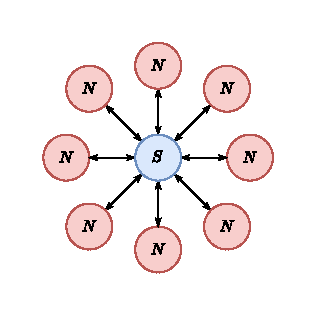
\includegraphics[width=\textwidth]{figures/topo-centralized}
    \caption{Centralized}
    \label{fig:cids.centralized}
  \end{subfigure}%
  \begin{subfigure}{.25\textwidth}
    \centering
    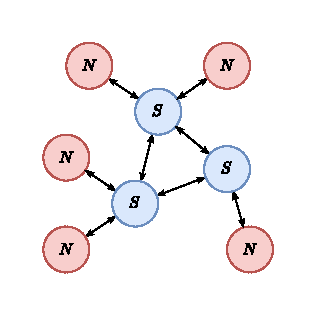
\includegraphics[width=\textwidth]{figures/topo-decentralized}
    \caption{Decentralized}
    \label{fig:cids.decentralized}
  \end{subfigure}%
  \begin{subfigure}{.25\textwidth}
    \centering
    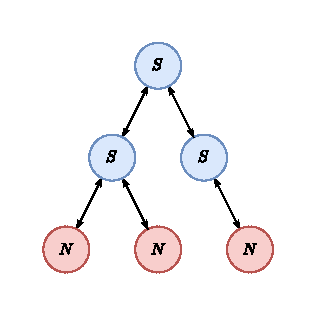
\includegraphics[width=\textwidth]{figures/topo-hierarchical}
    \caption{Hierarchical}
    \label{fig:cids.hierarchical}
  \end{subfigure}%
  \begin{subfigure}{.25\textwidth}
    \centering
    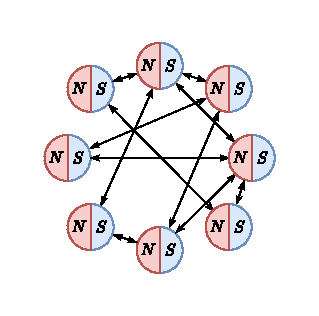
\includegraphics[width=\textwidth]{figures/topo-distributed}
    \caption{Distributed}
    \label{fig:cids.distributed}
  \end{subfigure}
  \caption[
    Different topologies for collaborative intrusion detection systems.
  ]{
    Different topologies for collaborative intrusion detection systems.
    Nodes are in red and marked as $N$, while servers are in blue and marked as $S$.
    Arrows represent connections between entities.
    \label{fig:cids.topoligies}
  } 
\end{figure}

The aforementioned literature identify three main types of topologies for \glspl{cids}: centralized, decentralized, and distributed.
The definitions of these topologies are not always consistent across the literature, especially between the terms \emph{decentralized}, \emph{hierarchical}, and \emph{distributed}.
For instance, \textcite{zhou_surveycoordinatedattacks_2010} consider a decentralized system as a system where each node is autonomous and can make decisions independently, while this definition matches the description of a distributed architecture in the work of \textcite{li_SurveyingTrustBasedCollaborative_2022}.

In this manuscript, we will use the definitions illustrated in \Cref{fig:cids.topoligies}.
It distinguishes two types of roles: \emph{nodes} ($N$) and \emph{servers} ($S$).
A node is a device that captures data, although it can also execute complementary tasks like preprocessing, feature extraction, or traffic analysis.
A server is a device that aggregates the data from the nodes and distributes instructions to them, as well as updates for the local detection algorithm.
The different topologies are defined as follows:
\begin{description}
  \item[Centralized] In a centralized architecture, a single server centralizes knowledge and distributes instructions to the nodes.
  \item[Decentralized] In a decentralized architecture, multiple servers coexist.
    Each server is responsible for a subset of the nodes, and they can share information between them.
  \item[Hierarchical] A hierarchical architecture is decentralized system where the servers are organized in a tree-like structure.
    Each server is responsible for a subset of the nodes, and they can forward information to their parent.
    Likewise, parents can distribute instructions and updates to their children so that they are disseminated throughout the hierarchy.
  \item[Distributed] In a distributed architecture, each node is autonomous and can make decisions independently.
    Both roles of nodes and servers coexist in the same entity.
    There are no servers anymore, and the node share information over a peer-to-peer network.
\end{description}

\Cref{fig:cids.topoligies} illustrates these topologies.
In the centralized architecture (\Cref{fig:cids.centralized}), all nodes are connected to a single server.
\Cref{fig:cids.decentralized} shows a standard example of a decentralized architecture.
\Cref{fig:cids.hierarchical,fig:cids.distributed} illustrate the specific cases of decentralized architectures: hierarchical and distributed, respectively.
The arrows between the different entities represent information exchange, although the nature of these exchanges can vary depending on the direction.
An arrow displayed as $N \rightarrow S$ can represent collected data, generated alerts, or requests for updates.
An arrow displayed as $S \rightarrow N$ can represent instructions or updates for the local detection algorithm or database.

\subsection{Challenges in Collaborative Intrusion Detection\label{sec:bg.collab.challenges}}

Collaborative intrusion detection faces challenges, including the \gls{spof} in a centralized architecture.
If the analysis is performed remotely, like in a \gls{soc} monitoring its consumers' infrastructures, a failure on the central server would hinder detection.
Fortunately, in knowledge-sharing scenarios, detection is (at least partially) performed locally, reducing the impact of a centralized failure.
Nonetheless, collaboration still relies on the availability of the central server.

\begin{challenge}
  \Glspl{cids} typically rely on a central server for coordination and updates, which represent a \acrfull{spof}.
  \label{chall:spof}
\end{challenge}

Another challenge in collaborative intrusion detection is the latency induced by propagating information over the network, especially under load.
The ENISA, the European Union Agency for Cybersecurity, defines the actionability of \gls{ti} as the fulfillment of five criteria: relevance, digestibility, accuracy, completeness, and timeliness~\cite{ENISA2014}.
It is the supporting architecture that provides the latter.
Because low-latency is crucial for actionable alerts locally, centrally analyzing the data increases the time between the event and its detection.

\begin{challenge}
  Centralized detection increases latency, which makes the shared knowledge less actionable.
  \label{chall:actionability}
\end{challenge}

Further, sharing data can represent a privacy risk for a company, as the data relevant for intrusion detection is likely to contain sensitive information~\cite{zhou_surveycoordinatedattacks_2010}.
Exposed information might reveal relevant insights to a competitor or an attacker.


\begin{challenge}
  \Glspl{cids} can expose sensitive information about the internals of a company.
  \label{chall:privacy}
\end{challenge}

A lot of other factors can impede collaboration.
For instance, stakeholders are often reluctant to share their information, fearing confidentiality and privacy issues (see \Cref{chall:privacy}), but most importantly the reputation loss that could result from a breach~\cite{pala_InformationSharingCybersecurity_2019}.
Cultural and language barriers can negatively affect the accuracy of the shared information, even though international collaboration is push by regulation, such as the NIS directives in Europe \cite{NIS_directive,NIS2}.
Finally, the balance between anonymity and trust must be taken into consideration to protect the participants without sacrificing the quality of the information~\cite{murdoch_AnonymityvsTrust_2015}.


\subsection{\Gls{cids} with \acrlong{ml}\label{sec:bg.collab.ml}}

Before the advent of \gls{fl}, the literature on \glspl{cids} leveraging \gls{ml}, or more generally data-mining techniques, was scarce~\cite{folino_Ensemblebasedcollaborative_2016}.
Existing solutions were mostly based sharing alerts for correlation or rules for misuse detection, or rely on a central server to perform learning tasks.
Nonetheless, a few works leveraged distributed learning techniques that remind of \gls{fl}, notably with the constraint of not being able to share data between the nodes.
For instance, \textcite{folino_ensemblebasedevolutionaryframework_2010} proposed a framework allowing distributed \gls{ids} nodes to train and exchange classifiers, before aggregating to build ensemble models.
However, most of the aforementioned reviews still identify data-mining and \gls{ml} techniques as a promising direction for \glspl{cids}.

\section{Fundamentals of Federated Learning\label{sec:bg.fl}}

Introduced in 2016 by \textcite{mcmahan_Communicationefficientlearningdeep_2017}, \acrfull{fl} changes the usual \gls{ml} paradigm where distributed data is centrally collected, curated, and processed on a dedicated server. 
Instead, \gls{fl} respects the decentralized nature of the data and rather brings model training to the data sources.
By alternating between training on local data and aggregating model updates, \gls{fl} enables the training of a shared model without the need to share the data itself.
This approach reveals itself as a promising solution to multiple challenges faced by traditional \gls{ml} systems, the two main ones being:
\begin{enumerate}
    \item Training models over massively distributed data sources, such as smartphones, wearables, or IoT devices; and
    \item Training models on sensitive data, such as medical records or financial transactions, while preserving privacy and confidentiality.
\end{enumerate}

Although the term \emph{Federated Learning} was introduced by \textcite{mcmahan_Communicationefficientlearningdeep_2017} to describe their approach focusing on distributed mobile devices, the literature has significantly broadened the definition of \gls{fl} to encompass a wide range of privacy-preserving distributed learning techniques.
Therefore, we prefer the definition introduced in 2021 by \textcite{kairouz_AdvancesOpenProblems_2021} and reiterated in \Cref{def:fl}.
The following sections introduce the fundamentals of \gls{fl}, with a focus on the \texttt{FedAvg} algorithm, the different types of \gls{fl}, and the question of data distribution.
Finally, we succinctly discuss the threats against \gls{fl}, with a focus on data poisoning attacks.
\Cref{tbl:notations} summarizes the notations used in this section, and throughout the manuscript.

\begin{definitionbox}{Federated Learning}{fl}
  \emph{Federated Learning} is a machine learning setting where multiple entities (clients) collaborate in solving a machine learning problem, under the coordination of a central server or service provider.
  Each client’s raw data is stored locally and not exchanged or transferred; instead, focused updates intended for immediate aggregation are used to achieve the learning objective. -- \textcite{kairouz_AdvancesOpenProblems_2021}

  \tcblower

  Formally, \gls{fl} seeks to minimize a objective function $f(\cdot)$\footnotemark, as:
  \begin{equation}
    \min_{w} f(w), \quad \text{where} \quad f(w) = \sum_{k=1}^{K} \rho_k f_k(w),
  \end{equation}
  where $w$ is the model parameters, $f_k(w)$ is the local objective function of client $k$, and $\rho_k$ is the weight of client $k$.

\end{definitionbox}

\footnotetext{Note that in the context of intrusion detection using \gls{ml}, the objective function $f(\cdot)$ is often a loss function $\mathcal{L}(\cdot)$ to minimize, such as mentioned in \Cref{sec:bg.ids.dl}.}

\begin{table}[ht]
  \centering
  \caption{Summary of Notations.\label{tbl:notations}}
  % LTeX: enabled=false

%\begin{tabularx}{\textwidth}{lX}
\begin{tabular}{ll}
  \toprule % ---------------------------------
  \textbf{Notation}                                                   & \textbf{Description} \\
  \midrule % ---------------------------------
  $K$                                                                 & Number of participants \\
  $P = \lbrace p_i | i \in \llbracket 1,K \rrbracket \rbrace$         & Set of all participants \\
  $C$                                                                 & Fraction of selected participants \\
  $d_k$                                                               & Local dataset of participant $p_k$ \\
  $D = \bigcup_{i=1}^K d_i$                                           & Union of all local datasets \\
  $X_i = \langle x_1, x_2, \dots, x_m \rangle$                        & Features of sample $i$ \\
  $Y_i$                                                               & Label enconding for sample $i$ \\
  $w_i^r$                                                             & Local model of the $k$-ith participant at round $r$ \\
  $W = (w_i^r | i \in \llbracket 1,K \rrbracket)$                     & Local models from participants at round $r$ \\
  $\bar{w}$                                                           & Aggregated model at round $r$ \\
  $L(w_i, d_i)$                                                       & Loss function for model $w_i$ on $d_i$ \\
  $\mathcal{E}$                                                       & Number of local epochs \\
  $\beta$                                                             & Batch size \\
  $\eta$                                                              & Learning rate \\
  \bottomrule % ---------------------------------
%\end{tabularx}
\end{tabular}
\end{table}


\subsection{The \texttt{FedAvg} Algorithm\label{sec:bg.fl.fedavg}}

\texttt{FedAvg} is the first and most popular algorithm for \gls{fl}.
The algorithm operates in rounds, noted $r$.
At each round $r$, an orchestrating server $S$ randomly selects $C \cdot K$ clients from a pool of participants $P$, with $K$ being the total number of participants and $C$ the fraction of clients selected with $0 < C \leq 1$.
The server then tasks each selected participant $p_k, k\in \llbracket 1,K \rrbracket$ to train a model $w_k^r$.
The round ends by the aggregation of the collected models into a new global model $\bar{w}^r$, which is redistributed to the clients as a starting point for the next round ($r+1$).

In essence, \texttt{FedAvg} is a distributed 2-level \gls{sgd} algorithm, where $C$ controls the \emph{global} batch size, and then each client $p_k$ uses a \emph{local} batch of size $\beta$ to compute a local update.
To train their model, the participants use a \gls{sgd}-based optimizer to minimize a objective function $f_k(w)$, which is the local loss function of client $p_k$ (see \Cref{def:fl}).
They compute the gradients of the loss function with respect to the model parameters, as:
\begin{equation}
  g_k^r = \nabla f_k(w_k^r),
\end{equation}
with is the results of the local optimization process.

In their original publication, \textcite{mcmahan_Communicationefficientlearningdeep_2017} introduce two algorithms for \gls{fl}: \texttt{FedSGD} and \texttt{FedAvg}.
\texttt{FedSGD} is a straightforward implementation of \gls{sgd} in a federated setting, where each client computes the gradients after one epoch and sends them to the server.
The server then aggregates the gradients and updates the global model.
With $D=\bigcup_{k=1}^K d_k$ being the union of all local datasets $d_k$, the server computes the new global model as:
\begin{equation}
  w^{r+1} = w^r - \eta \sum_{k=1}^{K} \frac{|d_k|}{|D|} g_k^r,
\end{equation}
where $\eta$ is the learning rate, and $|d_k|$ and $|D|$ are the sizes of the local dataset and the global dataset, respectively.

Based on the observation that there is no difference between averaging the gradients $g_k^r$ and updating the global model, or updating the model locally and then averaging the results, \textcite{mcmahan_Communicationefficientlearningdeep_2017} introduce \texttt{FedAvg}.
Indeed, the two operations are equivalent, as the following equation shows:
\begin{equation}
  w^{r+1} = w^r - \eta \sum_{k=1}^{K} \frac{|d_k|}{|D|} g_k^r = \sum_{k=1}^{K} \frac{|d_k|}{|D|} w_k^r,
\end{equation}
where $w_k^r$ is the model trained by client $p_k$ at round $r$.
This equivalence allows clients to train their models for multiple epochs before sending the results to the server, which reduces the communication overhead.
\Cref{alg:fedavg} summarizes the \texttt{FedAvg} algorithm.

This core idea, that \emph{averaging locally trained models iteratively converges towards an optimal model trained over distributed data}, is the foundation of \gls{fl}.

\begin{figure}
  \centering
  \begin{minipage}{.8\textwidth}
    
    \begin{algorithm}[H]
      \caption{
        \texttt{FedAvg}~\cite{mcmahan_Communicationefficientlearningdeep_2017}.
        The participants of $|P|$ are indexed by $p$, $C$ is the fraction of participants to be selected at each round, $\beta$ the local batch size, $\eta$ the learning rate, $\mathcal{E}$ the number of epochs, and $\nabla\mathcal{L}$ the gradients of the loss function $\mathcal{L}$.
        \label{alg:fedavg}
      }
      \begin{algorithmic}[1]
      
        \State Initialize $w_0$
        \For{each round $r = 1,2,\dots$}
          \State $ m \gets \Call{max}{C \cdot K, 1} $
          \State $ P^r \gets (\Call{SelectRandom}{m, P}) $
          \ForAll{$ p_k \in P^r $}
            \State $ w_k^r \gets \Call{ClientFit}{p_k, w^r} $
          \EndFor
          \State $ w^{r+1} \gets \sum_{k=1}^{K} \frac{|d_k|}{|D|} w_k^r $
        \EndFor
    
        \Statex
        \LComment{On client $p$.}
        \Function{ClientFit}{$p$, $\omega$} 
          \For{$ i \gets 1,\dots,\mathcal{E} $}
            \ForAll{$ b \in \Call{Split}{d_k, \beta} $}
              \State $ \omega \gets \omega - \eta \nabla \mathcal{L}(\omega,b) $
            \EndFor
          \EndFor
          \Statex
          \State \Return $\omega$
        \EndFunction
      \end{algorithmic}
    \end{algorithm}
  \end{minipage}
\end{figure}


\subsection{Types of Federated Learning\label{sec:bg.fl.types}}

As stated in the introduction of this section, the literature has broadened the scope of \gls{fl}, leading to different types of \gls{fl} depending on the context and the objectives of the federation.

\paragraph{Cross-device \vs Cross-silo Federated Learning}

The first notable distinction is between \gls{cdfl}, the context in which \gls{fl} was introduced, and \gls{csfl}.
The \emph{cross-device} settings concerns massively distributed devices which are typically low-power and resource-constrained, such as smartphones, wearables, or \gls{iot} devices.
Their number can range from thousands to billions, and they are often owned by different users.
Consequently, \gls{cdfl} often encounters challenges related to limited availability, reliability, and communication overhead, but offers scalability and adaptability.
In contrast, in \emph{cross-silo} settings, \gls{fl} operates within organizational boundaries or distinct data silos, where each silo represents a separate entity or institution.
Silos could correspond to different departments within a company, independent organizations, or even geographical regions.
\gls{csfl} typically implies organizations with more homogeneous capabilities and more data to train on.
Parties in cross-silo \gls{fl} are more likely to be reliable and consistently available for participation, as they are usually institutional entities with dedicated infrastructure and resources.
Yet, entities involved in \gls{csfl} also tend to have considerably greater discrepancies in terms of objectives and data-distributions, and sometimes even model architectures.


\paragraph{Horizontal \vs Vertical \gls{fl}}

\begin{figure}
  \centering
  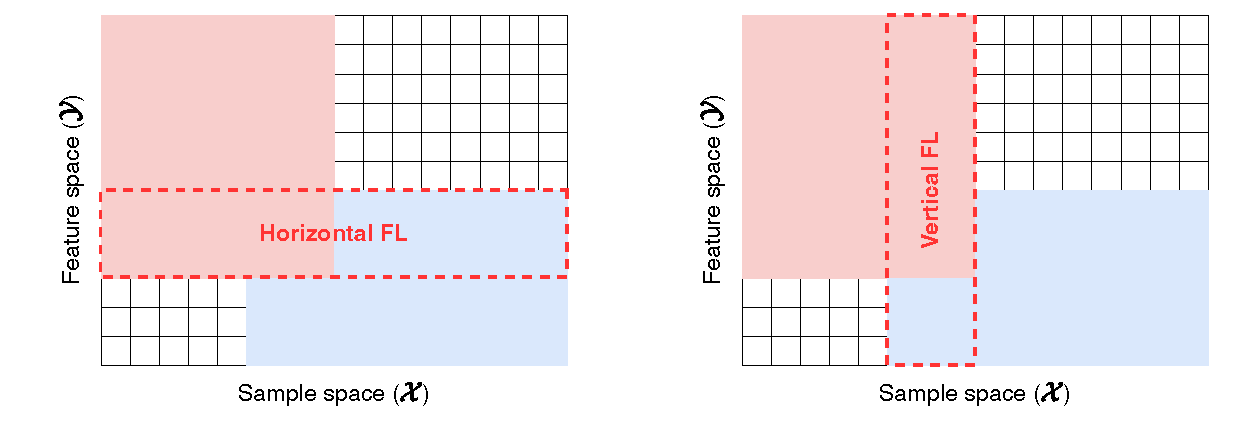
\includegraphics[width=.8\textwidth]{figures/horizontal-vertical.drawio.pdf}
  \caption{
    Horizontal \vs Vertical Federated Learning.
    In horizontal \gls{fl}, clients share the same features but not the same samples.
    In vertical \gls{fl}, clients share the same samples but not the same features.
    \label{fig:fl.horizontal-vertical}
  }
\end{figure}

Another major distinction in \gls{fl} is on along which axis the data is distributed.
In most application (notably in \gls{cdfl}), participants share the same features, but possess different samples.
This is referred to as \gls{hfl} by \textcite{yang_FederatedMachineLearning_2019}, and is illustrated in \Cref{fig:fl.horizontal-vertical}.
\Gls{hfl} particularly copes with \emph{ground-truth} issues (\Cref{chall:specificity}) by providing more data for the global model to be trained on.
Conversely, in \gls{vfl}, participants might have different views over the same data, \ie they share the same samples but not the same features.
This is particularly relevant in cross-silo applications, where different organizations might have access to different data sources, but observe the same events.
Finally, \textcite{yang_FederatedMachineLearning_2019} also consider \gls{ftl}, where participants share only a subset of both, features and samples.


\paragraph{Architecture Discrepancies}

Although \gls{fl}'s definition implies a client-server architecture, the literature has also explored other settings.
In the \emph{server-orchestrated} setting, the central server plays a pivotal role in distributing model parameters, orchestrating training rounds, and aggregating updates from individual devices.
This approach requires global coordination and synchronization, as all communication and aggregation activities are orchestrated by the server.
While server-orchestrated \gls{fl} offers centralized control and streamlined management, it also introduces potential single points of failure and scalability limitations due to the server's central role.
This is reminiscent of the centralized architecture mentioned in \Cref{sec:bg.collab,fig:cids.centralized} and comes with the same caveats.
Researchers have explored multiple alternatives to the server-orchestrated setting, such as hierarchical \gls{fl}~\cite{liu_ClientEdgeCloudHierarchicalFederated_2020} or fully decentralized \gls{fl} using gossip algorithms~\cite{tang_GossipFLDecentralizedFederated_2023}.
This decentralized approach eliminates single points of failure and allows for greater scalability, as communication and computation can be distributed across numerous devices.
However, fully decentralized \gls{fl} may face challenges related to coordination, consistency, and synchronization, especially in scenarios with a vast number of participating devices.


\subsection{The Question of Data Distribution\label{sec:bg.fl.data}}

% iid vs non-iid
% types of non-iid
% how to handle non-iid data
% - algos: FedProx, Fed+
% - data augmentation
% - client-side sampling
% - clustering (dedicated section in chap:radar)

The performance of \gls{fl} algorithms is highly dependent on the distribution of the data across the participants.
Almost by definition, data in \gls{fl} settings is \gls{niid}, as it is distributed across different devices or organizations.
However, the performance of \gls{fl} algorithms of the literature is often evaluated under the assumption that the data is \emph{iid}, which is rarely the case in practice.
This discrepancy between the theoretical assumptions and the practical reality is a significant challenge for \gls{fl}.

The literature has addressed the issue of \gls{niid} data in \gls{fl} from multiple angles.
First, some algorithms have been specifically designed to handle \gls{niid} data, such as \texttt{FedProx}~\cite{li_FederatedOptimizationHeterogeneous_2020} or \texttt{SCAFFOLD}~\cite{karimireddy_SCAFFOLDStochasticControlled_2020}.
Techniques such as client-side sampling, in which clients sample their data to match the global distribution, have also been proposed~\cite{han_HeterogeneousDataAwareFederated_2024}.
Finally, the literature has also explored clustering approaches to group client with model updates in communities, assuming that similar updates come from clients with similar data distributions~\cite{ye_PFedSAPersonalizedFederated_2023}.


\subsection{Threats against Federated Learning\label{sec:bg.fl.threats}}

% - Threats against FL
%   - Threats summary
%   - Focus on data poisoning
%     - Attacker modeling
%     - Attack vectors
%     - Mitigation strategies

The distributed nature of \gls{fl} opens the way to various attack vectors, which can be classified into two main categories: attacks against the federated model and attacks targeting the participants' privacy.
In the former, adversaries aim to alter the behavior of the global model, either to degrade its performance or to manipulate specific predictions.
In the latter, adversaries seek to infer sensitive information about the participants' data, such as inferring the presence of a specific sample in a participant's dataset.

Because the two categories have different objectives, and consequently different threat models, we focus on the former in this thesis.
Authors often refer to poisoning attacks in \gls{fl} as \emph{Byzantine} attacks, as they are analogous to the concept of Byzantine faults in distributed systems.
Likewise, the term \emph{Sybil attacks}~\cite{douceur_SybilAttack_2002} is frequently used to refer to the problem of \emph{colluding attackers}~\cite{fung_LimitationsFederatedLearning_2020}.

\paragraph{Attack vectors}

Poisoning attacks can be categorized into two main categories depending on the phase in which they are perpetrated: model-poisoning~\cite{bhagoji_AnalyzingFederatedLearning_2019} or data-poisoning~\cite{tolpegin_DataPoisoningAttacks_2020}.
Model-poisoning attacks aim at manipulating the model's parameters, usually during or after training, to deviate the aggregated model from the global optimum~\cite{fang_LocalModelPoisoning_2020}.
Data-poisoning attacks, on the other hand, happen before the training phase, and manipulate data samples to degrade performance, cause misclassification, or introduce backdoors~\cite{rodriguez-barroso_Surveyfederatedlearning_2023}.

Data poisoning attacks can be categorized into clean-label and label-flipping attacks.
Clean-label attacks manipulate the samples to be misclassified, either by adding new samples~\cite{zhang_Evaluationdatapoisoning_2022} or by modifying existing ones~\cite{merzouk_Parameterizingpoisoningattacks_2023}.
Label-flipping attacks, on the other hand, change the labels of the samples by flipping them to a different class~\cite{tolpegin_DataPoisoningAttacks_2020}: \ie, $y_{\text{src}} \rightarrow y_{\text{target}}$. 

\paragraph{Attack target}

Additionally, most poisoning attacks can be further separated into \emph{untargeted} and \emph{targeted} attacks.
Untargeted attacks randomly select samples to be manipulated, and are usually easier to detect as they have a higher impact on the model's performance.
Targeted attacks, on the other hand, select samples based on a specific criterion, such as the class to be targeted.
In a \gls{cids} context, targeted attacks can be used to introduce backdoors -- \ie, making a specific attack class be misclassified as benign -- or cause targeted misclassification.

\section{Conclusion\label{sec:bg.conclusion}}



